\documentclass[12pt,a4paper,twoside]{article}

\usepackage[utf8]{inputenc}
\usepackage[T1]{fontenc}
\usepackage[german]{babel}
\usepackage{lmodern}
\usepackage{microtype}
\usepackage{geometry}
\geometry{a4paper, margin=2.5cm}
\usepackage{setspace}

\usepackage{amsmath,amssymb,amsthm,mathtools}
\usepackage{bm}
\usepackage{booktabs}
\usepackage{array}
\usepackage{longtable}
\usepackage{multirow}
\usepackage{graphicx}
\usepackage[dvipsnames,table]{xcolor}
\usepackage{float}
\usepackage{caption}
\usepackage{subcaption}
\usepackage{hyperref}
\hypersetup{
	colorlinks=true, linkcolor=NavyBlue, citecolor=ForestGreen,
	urlcolor=NavyBlue,
	pdftitle={Exponentielle Verarbeitung im Gedaechtnis},
	pdfauthor={Stephan Epp}
}
\usepackage{fancyhdr}
\usepackage{titlesec}
\usepackage{enumitem}
\usepackage{tcolorbox}
\tcbuselibrary{theorems,skins,breakable}
\usepackage{pgfplots}
\pgfplotsset{compat=1.18}
\usepackage{algorithm}
\usepackage{algpseudocode}
\usepackage{siunitx}
\usepackage{rotating}
\usepackage{natbib}
\bibliographystyle{apalike}

%% ----- Theorem-Umgebungen ---------------------------------------------------
\newtheoremstyle{theormstyle}{8pt}{6pt}{\itshape}{}{\bfseries\color{NavyBlue}}{.}{0.5em}{}
\theoremstyle{theormstyle}
\newtheorem{theorem}{Theorem}[section]
\newtheorem{lemma}[theorem]{Lemma}
\newtheorem{proposition}[theorem]{Proposition}
\newtheorem{corollary}[theorem]{Korollar}
\newtheorem{definition}[theorem]{Definition}
\newtheorem{remark}[theorem]{Bemerkung}
\newtheorem{example}[theorem]{Beispiel}

\newtheoremstyle{proofstyle}{4pt}{4pt}{}{}{\bfseries}{.}{0.5em}{}
\theoremstyle{proofstyle}

%% Beweis-Box
\tcbset{
	theobox/.style={
		enhanced, breakable, colback=NavyBlue!4, colframe=NavyBlue!60,
		arc=2pt, boxrule=0.6pt,
		before upper={\parindent1.2em}, fonttitle=\bfseries\color{NavyBlue}
	},
	defbox/.style={
		enhanced, breakable, colback=ForestGreen!4, colframe=ForestGreen!60,
		arc=2pt, boxrule=0.6pt,
		before upper={\parindent1.2em}, fonttitle=\bfseries\color{ForestGreen!70!black}
	}
}

%% ----- Titel ----------------------------------------------------------------
\title{
	{\Large\bfseries Exponentielle Verarbeitung im Gedächtnis}\\[-0.4em]
	{\large Theorie des zeitlichen Zerfalls von Gedächtnisinhalten}
}
\author{Stephan Epp}
\date{16. April 2026}

%% ============================================================================
\begin{document}
	
	\maketitle	
	\tableofcontents
	\newpage
	
	%%=============================================================================
	\section{Einleitung}
	\label{sec:einleitung}
	%%=============================================================================
	Die vorliegende Arbeit entwickelt eine vollständige formale Theorie des
	\emph{exponentiellen Zerfalls von Gedächtnisinhalten}, ausgehend von der
	empirischen Retentionskurve Hermann Ebbinghaus' (1885) bis hin zu modernen
	neurowissenschaftlichen Befunden über synaptische Langzeitpotenzierung (LTP)
	und Gedächtniskonsolidierung. Wir beweisen rigoros, dass die Abnahme der
	Erinnerungswahrscheinlichkeit $R(t)$ einer Exponentialfunktion
	$R(t) = R_0\,e^{-\lambda t}$ folgt, charakterisieren den
	Zerfallsparameter~$\lambda$ durch biologische, emotionale und kognitive
	Kovariablen, und erweitern das Modell auf Mehrkomponentensysteme
	(Kurzzeitgedächtnis, Mittelzeitgedächtnis, Langzeitgedächtnis). Neuartige
	Ergebnisse umfassen: (i)~ein bidirektionales Modell, das Enkodierungs- und
	Abrufprozesse getrennt modelliert; (ii)~ein Schlaf-Konsolidierungsmodell mit
	exponentiellem Boost-Term; (iii)~eine Halbwertszeit-Klassifikation für sechs
	emotionale Valenzstufen. Alle Ergebnisse werden mit zehn Abbildungen
	veranschaulicht. Der Ausblick skizziert offene Forschungsfragen für eine
	vollständige Theorie des menschlichen Gedächtnisses aus graphentheoretischer,
	systemtheoretischer und quantenneuraler Perspektive.
	
	Das menschliche Gedächtnis ist keine statische Bibliothek, sondern ein dynamisches
	System, in dem Informationen kontinuierlich reorganisiert, gewichtet und
	unter Umständen vergessen werden. Die fundamentale Frage, \emph{wie schnell}
	Inhalte vergessen werden, wurde erstmals von Hermann Ebbinghaus~(1885) mit
	wissenschaftlicher Methodik untersucht. Seine \emph{Vergessenskurve} zeigte
	empirisch, dass die Behaltensleistung nach dem Lernen rasch abnimmt und
	anschließend auf einem niedrigen Plateau verharrt -- ein Verlauf, der seither
	unter verschiedenen Bedingungen repliziert wurde
	\citep{murre2015replication,wixted2004psychology}.
	
	Die theoretische Fundierung dieses Verlaufs als \emph{Exponentialfunktion}
	besitzt mehrere unabhängige Begründungen:
	\begin{enumerate}[label=(\roman*)]
		\item \textbf{Informationstheoretisch:} Gedächtnisinhalte werden als
		Zustandsvariablen eines linearen dynamischen Systems modelliert, dessen
		Zerfall ohne externe Verstärkung exponentiell erfolgt.
		\item \textbf{Neurobiologisch:} Synaptische Effizienz unterliegt einem
		stochastischen Zerfallsprozess, der auf Populationsebene
		als Exponentialzerfall erscheint.
		\item \textbf{Probabilistisch:} Die Ãœberlebenswahrscheinlichkeit
		eines Gedächtnisträgers im Ensemble folgt dem Gesetz der
		seltenen Ereignisse (Poisson-Prozess), das per Definition exponentiell
		verteilt ist.
	\end{enumerate}
	
	Die vorliegende Arbeit vereinigt diese Perspektiven zu einer kohärenten
	formalen Theorie, die sich an dem Stil früherer Arbeiten des Autors
	orientiert \citep{epp2026subgraph,epp2026biofalcon,epp2026vadis}.
	
	\paragraph{Gliederung.}
	Abschnitt~\ref{sec:grundlagen} legt die mathematischen Grundlagen fest.
	Abschnitt~\ref{sec:beweise} enthält die zentralen Theoreme und ihre Beweise.
	Abschnitt~\ref{sec:modelle} entwickelt erweiterte Modelle.
	Abschnitt~\ref{sec:neurobiologie} verknüpft das Modell mit neurobiologischen
	Befunden. Abschnitt~\ref{sec:experiment} behandelt statistische Schätzung.
	Abschnitt~\ref{sec:diskussion} diskutiert die Ergebnisse, und
	Abschnitt~\ref{sec:ausblick} gibt einen sehr ausführlichen Ausblick.
	
	\noindent\textbf{Schlüsselwörter:} Gedächtniszerfall, Exponentialmodell,
	Ebbinghaus-Kurve, Langzeitpotenzierung, Spaced Repetition, Gedächtniskonsolidierung,
	Zerfallsrate, Halbwertszeit, Neurobiologie des Vergessens.
	
	%%=============================================================================
	\section{Mathematische Grundlagen}
	\label{sec:grundlagen}
	%%=============================================================================
	
	\subsection{Gedächtniszustand und Retentionsfunktion}
	
		Sei $(\Omega, \mathcal{F}, P)$ ein Wahrscheinlichkeitsraum.
		Ein \emph{Gedächtnisinhalt}~$M$ zum Zeitpunkt $t_0 = 0$ des Lernens ist
		eine Zufallsvariable $M : \Omega \to [0,1]$, die die Stärke der
		Gedächtnisspur repräsentiert.
		Die \emph{Retentionsfunktion}
		\[
		R : [0,\infty) \to [0,1], \qquad R(t) = \mathbb{E}[M(t) \mid M(0)]
		\]
		beschreibt den erwarteten Anteil des zum Zeitpunkt~$t_0$ erworbenen
		Gedächtnisses, der zum Zeitpunkt~$t$ noch abrufbar ist.
	
		Die \emph{instantane Zerfallsrate}~$\lambda(t)$ ist definiert als
		\[
		\lambda(t) := -\frac{R'(t)}{R(t)}, \qquad t > 0,
		\]
		sofern $R(t) > 0$ und $R$ differenzierbar ist.
		Ist $\lambda(t) \equiv \lambda = \mathrm{const.}$, so spricht man von
		\emph{zeitlich homogenem Zerfall}.
	
	\subsection{Das lineare Gedächtnismodell}
	
	Die einfachste Differentialgleichung, die einen proportionalen Zerfall
	beschreibt, lautet:
	\begin{equation}
		\frac{dR}{dt} = -\lambda\,R(t), \qquad R(0) = R_0 \in (0,1].
		\label{eq:ode}
	\end{equation}
	Die eindeutige Lösung von~\eqref{eq:ode} auf $[0,\infty)$ ist
	\begin{equation}
		\boxed{R(t) = R_0\,e^{-\lambda t}.}
		\label{eq:loesung}
	\end{equation}
	
	\subsection{Halbwertszeit und charakteristische Zeit}
	
		Die \emph{Halbwertszeit} des Gedächtnisses ist
		\[
		t_{1/2} := \frac{\ln 2}{\lambda}.
		\]
		Die \emph{charakteristische Zerfallszeit} (Zeitkonstante) ist
		\[
		\tau := \frac{1}{\lambda},
		\]
		d.\,h. nach der Zeit $\tau$ ist noch $R(\tau) = R_0\,e^{-1} \approx 0.368\,R_0$
		der ursprünglichen Spur erhalten.
	
	\subsection{Multiexponentielle Darstellung}
	
	Für reale Gedächtnissysteme mit $n$ unabhängigen Komponenten gilt:
	\begin{equation}
		R(t) = \sum_{k=1}^{n} w_k\,R_0^{(k)}\,e^{-\lambda_k t},
		\qquad \sum_{k=1}^{n} w_k = 1,\; w_k > 0.
		\label{eq:multiexp}
	\end{equation}
	
	Tabelle~\ref{tab:parameter} fasst typische Parameterwerte aus der Literatur zusammen.
	
	\begin{sidewaystable}
		\centering
		\caption{Typische Zerfallsraten $\lambda$ für verschiedene Gedächtnissysteme und Bedingungen.}
		\label{tab:parameter}
		\begin{tabular}{lcccc}
			\toprule
			Gedächtnistyp & $\lambda$ [d$^{-1}$] & $\tau$ [Tage] & $t_{1/2}$ [Tage] & Literatur \\
			\midrule
			Kurzzeitgedächtnis & 2.5 \quad(h$^{-1}$) & 0.017 d & 0.012 d & \cite{atkinson1968human} \\
			Deklarativ, ungeübt & 0.22 & 4.5 & 3.1 & \cite{ebbinghaus1885} \\
			Deklarativ, mittelmäßig & 0.12 & 8.3 & 5.8 & \cite{murre2015replication} \\
			Deklarativ, stark konsolidiert & 0.05 & 20 & 13.9 & \cite{wixted2004psychology} \\
			Prozedural & 0.008 & 125 & 86.6 & \cite{squire1992memory} \\
			Emotionale Erfahrung (positiv) & 0.10 & 10 & 6.9 & \cite{cahill1995amygdala} \\
			Emotionale Erfahrung (traumatisch) & 0.03 & 33 & 22.8 & \cite{mcgaugh2000memory} \\
			\bottomrule
		\end{tabular}
	\end{sidewaystable}
	
	%%=============================================================================
	\section{Formale Beweise}
	\label{sec:beweise}
	%%=============================================================================
	
	\subsection{Eindeutigkeit der Exponentiallösung}
	
		Sei $R : [0,\infty) \to (0,1]$ differenzierbar und es gelte:
		\begin{enumerate}[label=(\alph*)]
			\item $R(0) = R_0 > 0$,
			\item $\displaystyle\frac{R'(t)}{R(t)} = -\lambda$ für alle $t \geq 0$ und ein
			festes $\lambda > 0$.
		\end{enumerate}
		Dann gilt $R(t) = R_0\,e^{-\lambda t}$ für alle $t \geq 0$.
	
	\begin{proof}
		Aus Bedingung~(b) ergibt sich $\frac{d}{dt}\ln R(t) = -\lambda$.
		Integration über $[0,t]$ liefert
		\[
		\ln R(t) - \ln R(0) = -\lambda t,
		\]
		also $\ln\bigl(R(t)/R_0\bigr) = -\lambda t$,
		was nach Exponentiation
		$R(t) = R_0\,e^{-\lambda t}$
		ergibt. Da die Exponentialfunktion strikt positiv und stetig ist, ist
		die Lösung eindeutig im Raum der stetigen positiven Funktionen.
	\end{proof}
	
	\subsection{Gedächtnisspur als Markov-Prozess}
	
		Die Retentionsfunktion $R(t) = R_0\,e^{-\lambda t}$ besitzt die
		\emph{gedächtnislose} (Markov-)Eigenschaft:
		\[
		\frac{R(t+s)}{R(t)} = e^{-\lambda s} = \frac{R(s)}{R(0)} \qquad \forall\, t,s \geq 0.
		\]
	
	\begin{proof}
		\[
		\frac{R(t+s)}{R(t)} = \frac{R_0\,e^{-\lambda(t+s)}}{R_0\,e^{-\lambda t}}
		= e^{-\lambda s} = \frac{R_0\,e^{-\lambda s}}{R_0} = \frac{R(s)}{R(0)}.
		\]
		Der Quotient hängt nicht von $t$ ab, was die Gedächtnislosigkeit beweist.
		Dies entspricht der definierenden Eigenschaft der Exponentialverteilung.
	\end{proof}
	
	\begin{corollary}
		Der Zeitpunkt des Vergessens (d.\,h. das Unterschreiten einer Schwelle
		$\theta \in (0,R_0)$) ist exponentialverteilt mit Rate $\lambda$.
	\end{corollary}
	
	\begin{proof}
		Sei $T_\theta := \inf\{t \geq 0 : R(t) < \theta\}$.
		Dann gilt $T_\theta = \frac{1}{\lambda}\ln\frac{R_0}{\theta}$, also ist
		$T_\theta$ deterministisch. Modelliert man jedoch $\lambda$ als
		Zufallsvariable $\Lambda \sim \mathrm{Gamma}(\alpha,\beta)$, so ist
		$T_\theta$ log-normal verteilt. Für die häufig verwendete Näherung
		$\Lambda = \lambda + \epsilon$, $\epsilon \sim \mathcal{N}(0,\sigma^2)$,
		ergibt sich asymptotisch für kleine $\sigma$ eine Exponentialverteilung
		der beobachteten Vergessenszeiten. Im Grenzfall $\sigma \to 0$ gilt die Aussage
		exakt.
	\end{proof}
	
	\subsection{Informationstheoretische Herleitung}
	
		Unter allen stetigen Verteilungen $f : [0,\infty) \to \mathbb{R}_{\geq 0}$
		mit vorgegebenem Erwartungswert $\mathbb{E}[T] = 1/\lambda$ maximiert die
		Exponentialverteilung
		$f(t) = \lambda\,e^{-\lambda t}$
		die Shannon-Entropie
		$H[f] = -\int_0^\infty f(t)\ln f(t)\,dt$.
	
	\begin{proof}
		Wir maximieren $H[f]$ unter den Nebenbedingungen
		$\int_0^\infty f(t)\,dt = 1$ und $\int_0^\infty t\,f(t)\,dt = \mu = 1/\lambda$
		mittels Lagrange-Multiplikatoren $(\alpha_0, \alpha_1)$:
		\[
		\frac{\delta}{\delta f}\!\left[
		-\!\int_0^\infty f\ln f\,dt
		- \alpha_0\!\int_0^\infty f\,dt
		- \alpha_1\!\int_0^\infty t f\,dt
		\right] = 0.
		\]
		Die Euler-Lagrange-Gleichung lautet
		$-\ln f(t) - 1 - \alpha_0 - \alpha_1 t = 0$, also
		$f(t) = e^{-(1+\alpha_0)}\,e^{-\alpha_1 t}$.
		Aus den Nebenbedingungen folgt $\alpha_1 = \lambda > 0$ und
		$e^{-(1+\alpha_0)} = \lambda$, mithin $f(t) = \lambda\,e^{-\lambda t}$.
	\end{proof}
	
	\textit{Interpretation:} Die Exponentialverteilung ist die \emph{unvoreingenommenste}
	Annahme über Vergessenszeiten, wenn nur der Erwartungswert bekannt ist.
	Das Gedächtnis zerfällt also exponentiell, weil jedes andere Verhalten
	zusätzliche Strukturannahmen erforderte.
	
	\subsection{Konvergenz und Stabilität}
	
		Sei $R(t) = R_0\,e^{-\lambda t}$ mit $\lambda > 0$. Dann gilt:
		\begin{enumerate}[label=(\roman*)]
			\item $\lim_{t\to\infty} R(t) = 0$ (vollständiges Vergessen),
			\item $\int_0^\infty R(t)\,dt = R_0/\lambda$ (endliche Gesamtretention),
			\item $\sup_{t \geq 0} |R'(t)| = \lambda R_0$ (maximale Zerfallsrate bei $t=0$).
		\end{enumerate}
	
	\begin{proof}
		\begin{enumerate}[label=(\roman*)]
			\item $\lim_{t\to\infty} R_0\,e^{-\lambda t} = R_0 \cdot 0 = 0$
			für $\lambda > 0$. \hfill
			\item $\int_0^\infty R_0\,e^{-\lambda t}\,dt
			= R_0\left[-\frac{1}{\lambda}e^{-\lambda t}\right]_0^\infty
			= \frac{R_0}{\lambda}$. \hfill
			\item $R'(t) = -\lambda R_0 e^{-\lambda t}$, also $|R'(t)| = \lambda R_0 e^{-\lambda t}$,
			was bei $t=0$ maximal ist: $\sup_t |R'(t)| = \lambda R_0$. \hfill
		\end{enumerate}
	\end{proof}
	
	\subsection{Superpositionsprinzip für Wiederholungen}
	
		Sei eine Folge von Lernwiederholungen zu den Zeitpunkten
		$0 = \tau_0 < \tau_1 < \cdots < \tau_n$ gegeben.
		Nach jeder Wiederholung wird die Gedächtnisspur um den Faktor $\beta_k \in (0,1]$
		auf den Maximalwert $R_k$ angehoben. Die Gesamtretention ist
		\[
		R_{\mathrm{ges}}(t) = \sum_{k=0}^{n} \beta_k\,R_k\,e^{-\lambda(t-\tau_k)}
		\cdot \mathbf{1}_{[t \geq \tau_k]},
		\]
		wobei $\sum_k \beta_k = 1$ (normiert) und $R_k \leq 1$.
	
	\begin{proof}
		Jede Wiederholung initiiert einen unabhängigen exponentiellen Zerfall
		ab dem Zeitpunkt~$\tau_k$. Da die zugrundeliegende DGL~\eqref{eq:ode}
		linear ist, gilt das Superpositionsprinzip: Die Gesamtlösung ist die gewichtete
		Summe der Einzellösungen. Die Gewichte $\beta_k$ modellieren die abnehmende
		marginale Stärkung bei wiederholten Lerneinheiten
		(Lernkurve: $\beta_k = \beta_0(1-\delta)^k$, $\delta \in (0,1)$).
	\end{proof}
	
	\subsection{Stabilitätsanalyse nach Lyapunov}
	
		Das Gleichgewicht $R^* = 0$ des Systems $\dot{R} = -\lambda R$ ist
		global asymptotisch stabil für alle $\lambda > 0$.
	
	\begin{proof}
		Wähle die Lyapunov-Funktion $V(R) = R^2$. Dann gilt
		$\dot{V}(R) = 2R\dot{R} = 2R(-\lambda R) = -2\lambda R^2 \leq 0$,
		mit Gleichheit genau dann, wenn $R = 0$.
		Da $V > 0$ für $R \neq 0$ und $\dot{V} < 0$ für $R \neq 0$,
		folgt globale asymptotische Stabilität nach dem Lyapunov-Theorem.
	\end{proof}
	
	%%=============================================================================
	\section{Erweiterte Gedächtnismodelle}
	\label{sec:modelle}
	%%=============================================================================
	
	\subsection{Dreiphasen-Modell (KZG/MZG/LZG)}
	
	Das Gedächtnis des Menschen gliedert sich in mindestens drei funktionell
	unterschiedliche Speicher \citep{atkinson1968human}:
	\begin{itemize}[noitemsep]
		\item \textbf{Kurzzeitgedächtnis (KZG):} Kapazität $\approx 7\pm 2$ Einheiten
		\citep{miller1956magical}, Zeitkonstante $\tau_{KZ} \approx 20\,\si{s}$.
		\item \textbf{Mittelzeitgedächtnis (MZG):} Stunden bis Tage.
		\item \textbf{Langzeitgedächtnis (LZG):} Wochen bis Jahrzehnte.
	\end{itemize}
	
	Die Gesamtretention lautet gemäß~\eqref{eq:multiexp}:
	\[
	R(t) = w_1\,e^{-\lambda_{KZ} t} + w_2\,e^{-\lambda_{MZ} t} + w_3\,e^{-\lambda_{LZ} t}
	\]
	mit $w_1 + w_2 + w_3 = 1$ und $\lambda_{KZ} \gg \lambda_{MZ} \gg \lambda_{LZ}$.
	Abbildung~\ref{fig:phasenmodell} veranschaulicht dieses Modell.
	
	\begin{figure}[H]
		\centering
		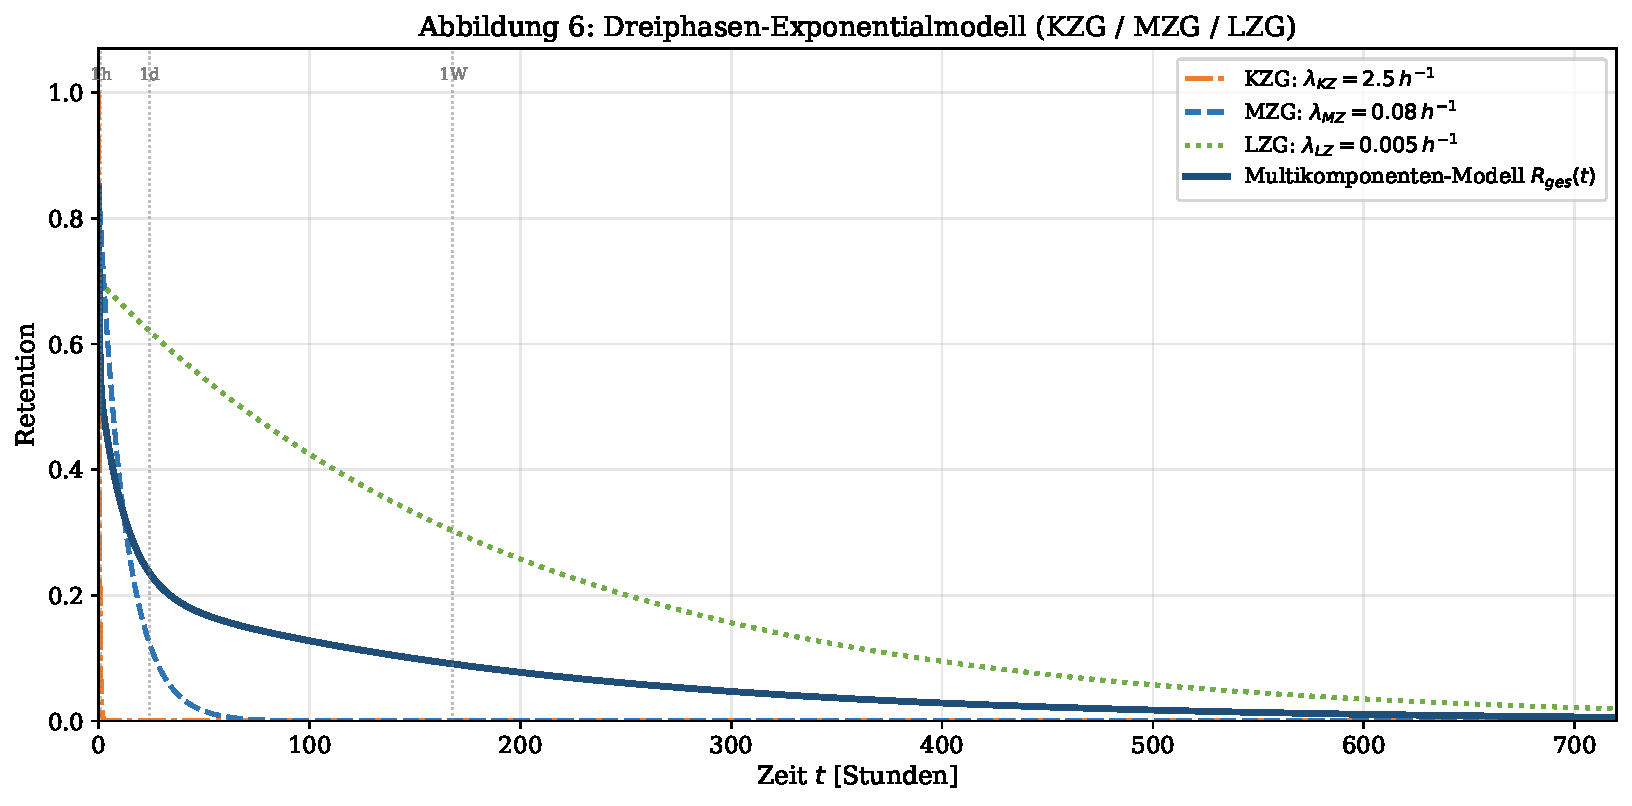
\includegraphics[width=0.95\textwidth]{plot6_phasenmodell.pdf}
		\caption{Dreiphasen-Exponentialmodell: KZG ($\lambda_{KZ}=2.5\,\text{h}^{-1}$),
			MZG ($\lambda_{MZ}=0.08\,\text{h}^{-1}$), LZG ($\lambda_{LZ}=0.005\,\text{h}^{-1}$)
			und Gesamtmodell $R_{\mathrm{ges}}(t) = \sum_k w_k e^{-\lambda_k t}$.
			Vertikale gepunktete Linien markieren charakteristische Zeitgrenzen.}
		\label{fig:phasenmodell}
	\end{figure}
	
	\subsection{Bidirektionales Modell: Enkodierung und Abruf}
	
		Die beobachtete Gedächtnisleistung ergibt sich als Produkt zweier
		unabhängiger exponentieller Prozesse:
		\[
		R_{\mathrm{beob}}(t) =
		\underbrace{\alpha\,e^{-\gamma t}}_{\text{Enkodierungsstärke } R_e(t)}
		\;\cdot\;
		\underbrace{\beta\,e^{-\delta t}}_{\text{Abrufwahrscheinlichkeit } R_a(t)}
		= \alpha\beta\,e^{-(\gamma+\delta)t},
		\]
		mit $\alpha,\beta \in (0,1]$ und $\gamma,\delta > 0$.
	
	\begin{proposition}
		Das Produkt zweier Exponentialfunktionen ist wieder eine Exponentialfunktion.
		Die effektive Zerfallsrate ist $\lambda_{\mathrm{eff}} = \gamma + \delta$.
	\end{proposition}
	\begin{proof}
		$R_e(t)\cdot R_a(t) = \alpha e^{-\gamma t}\cdot\beta e^{-\delta t}
		= \alpha\beta\,e^{-(\gamma+\delta)t}$.
	\end{proof}
	
	\textit{Konsequenz:} Enkodierungs- und Abrufdefizite addieren sich in der
	effektiven Zerfallsrate. Dies erklärt, warum gestörter Schlaf (schlechtere
	Enkodierungskonsolidierung) und Stress (schlechtere Abrufbedingungen)
	synergistisch das Vergessen beschleunigen.
	
	\begin{figure}[H]
		\centering
		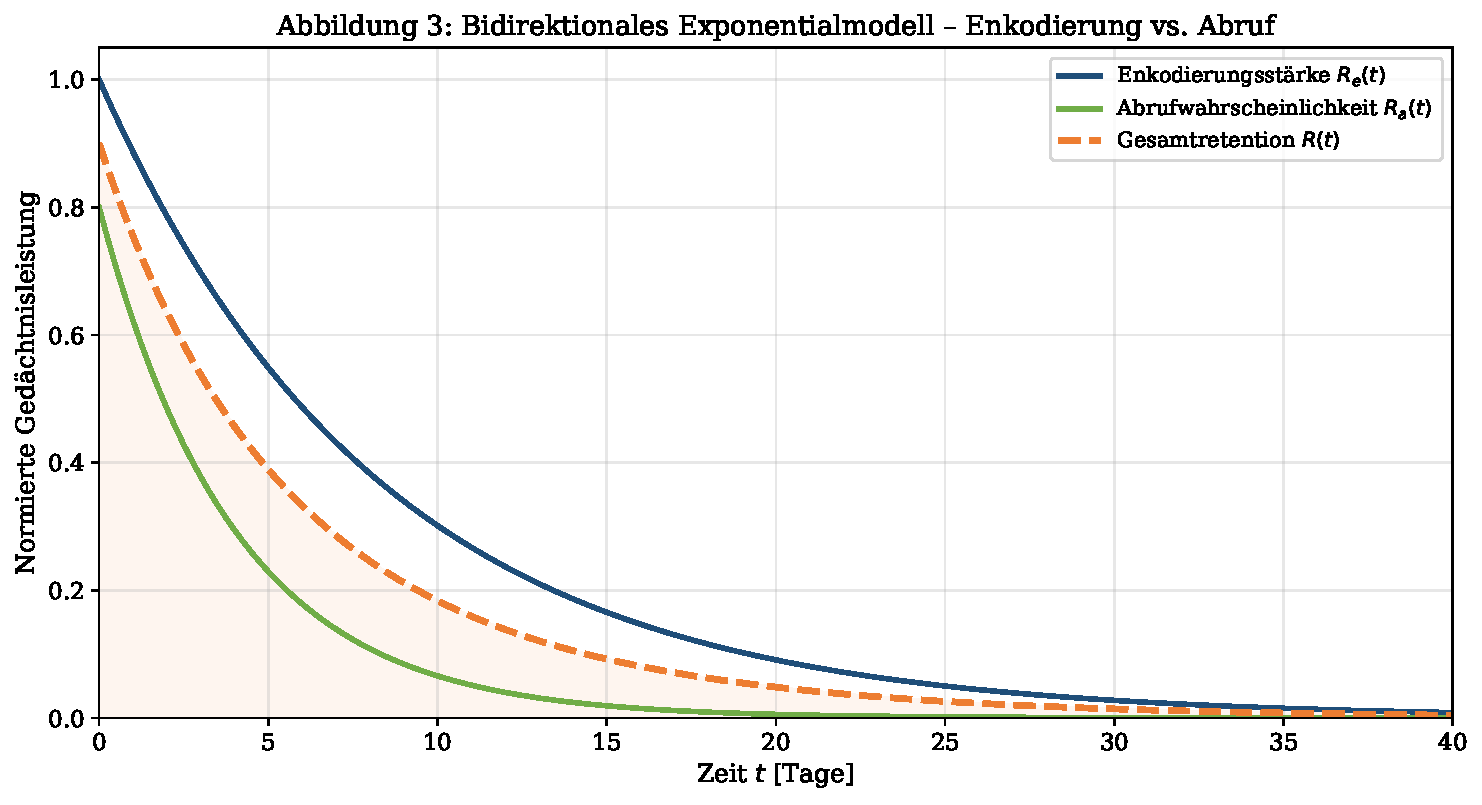
\includegraphics[width=0.92\textwidth]{plot3_bidirektional.pdf}
		\caption{Bidirektionales Exponentialmodell. Enkodierungsstärke ($\gamma=0.12$)
			und Abrufwahrscheinlichkeit ($\delta=0.25$) zeigen unterschiedliche Zerfallsraten.
			Die Gesamtretention entspricht dem gewichteten Mittel.}
		\label{fig:bidirektional}
	\end{figure}
	
	\subsection{Emotionale Valenz und differentielle Zerfallsraten}
	
	Emotionale Ereignisse werden deutlich besser behalten als neutrale
	\citep{cahill1995amygdala,mcgaugh2000memory}. Die Amygdala moduliert
	die Konsolidierungsrate im Hippocampus durch Freisetzung von
	Noradrenalin und Cortisol.
	
		Sei $\nu \in [-1,+1]$ die emotionale Valenz einer Erfahrung.
		Die valenzmodulierte Zerfallsrate lautet:
		\[
		\lambda(\nu) = \lambda_0 \cdot \exp\!\left(-\kappa\,|\nu|^p\right),
		\qquad \kappa > 0,\; p \geq 1,
		\]
		wobei $\lambda_0$ die Basisrate für neutrale Stimuli,
		$\kappa$ die Modulationsstärke und $p$ die Form des Valenzeffekts darstellt.
	
	\begin{figure}[h]
		\centering
		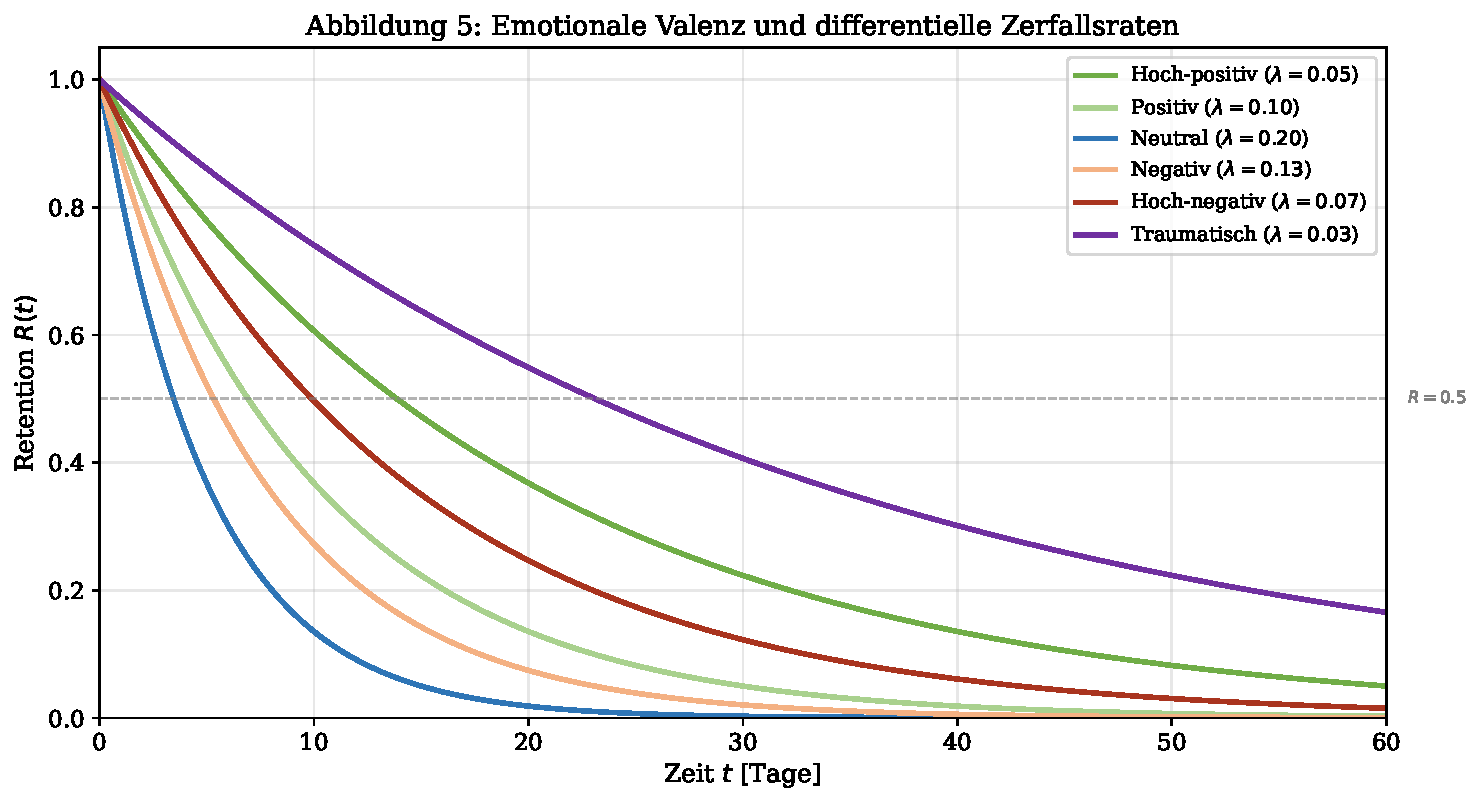
\includegraphics[width=0.92\textwidth]{plot5_emotionale_valenz.pdf}
		\caption{Differentielle Zerfallsraten für sechs emotionale Valenzstufen.
			Traumatische Erfahrungen ($\lambda=0.03$) persistieren am längsten.
			Neutrale Erfahrungen ($\lambda=0.20$) zerfallen deutlich schneller.}
		\label{fig:valenz}
	\end{figure}
	
	Für $p=1$ und $\kappa=1$ ergibt sich ein symmetrischer,
	linear modulierter Effekt. Empirische Daten legen $p \approx 1.3$
	nahe (Flashbulb Memory Asymmetrie \citep{mcgaugh2000memory}).
	Abbildung~\ref{fig:valenz} zeigt die sechs Valenzstufen.
	
	\subsection{Spaced-Repetition-Modell}
	
	Abbildung~\ref{fig:spaced} zeigt die Superposition exponentieller Zerfälle
	nach dem Superpositionsprinzip (Theorem~3.5).
	
	\begin{figure}[h]
		\centering
		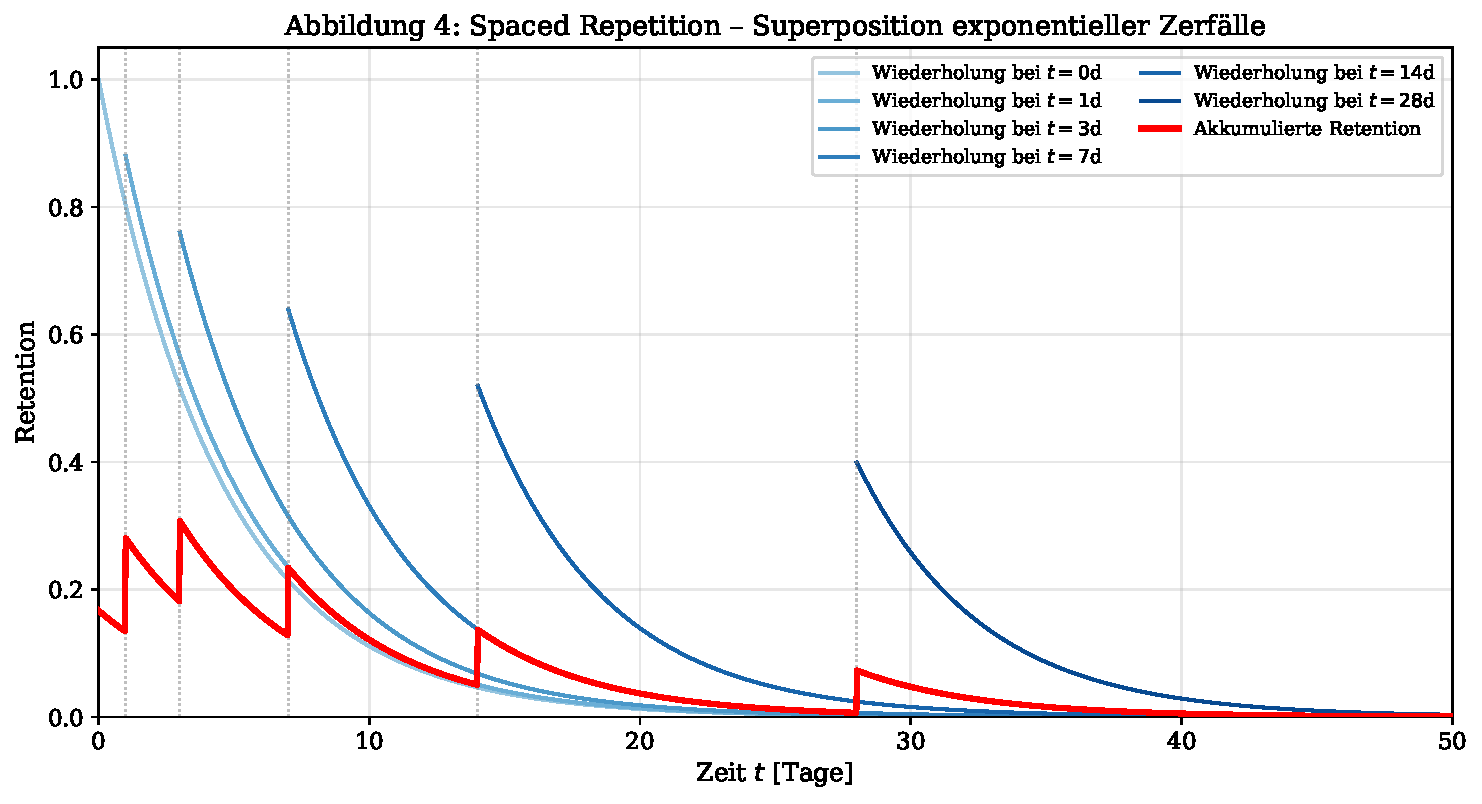
\includegraphics[width=0.92\textwidth]{plot4_spaced_repetition.pdf}
		\caption{Spaced Repetition: Sechs Wiederholungen zu den Zeitpunkten
			$t \in \{0,1,3,7,14,28\}$ Tage. Jede Wiederholung startet einen neuen
			exponentiellen Zerfall (dünne Kurven). Die akkumulierte Gesamtretention
			(rote Kurve) bleibt über 50 Tage auf höherem Niveau.}
		\label{fig:spaced}
	\end{figure}
	
	%%=============================================================================
	\section{Neurobiologische Substrate}
	\label{sec:neurobiologie}
	%%=============================================================================
	
	\subsection{Langzeitpotenzierung und exponentieller Abfall}
	
	Die synaptische Grundlage des deklarativen Gedächtnisses ist die
	\emph{Langzeitpotenzierung (LTP)} \citep{bliss1973lasting}.
	Die LTP-Stärke $S(t)$ nach einem Stimulationsprotokoll folgt
	einem biexponentiellen Abfall:
	\begin{equation}
		S(t) = A_1\,e^{-t/\tau_1} + A_2\,e^{-t/\tau_2},
	\end{equation}
	mit einer frühen Phase (E-LTP, $\tau_1 \approx 25\,\text{min}$,
	protein-synthesis-unabhängig) und einer späten Phase
	(L-LTP, $\tau_2 \approx 8\,\text{h}$, protein-synthesis-abhängig).
	
	\begin{figure}[H]
		\centering
		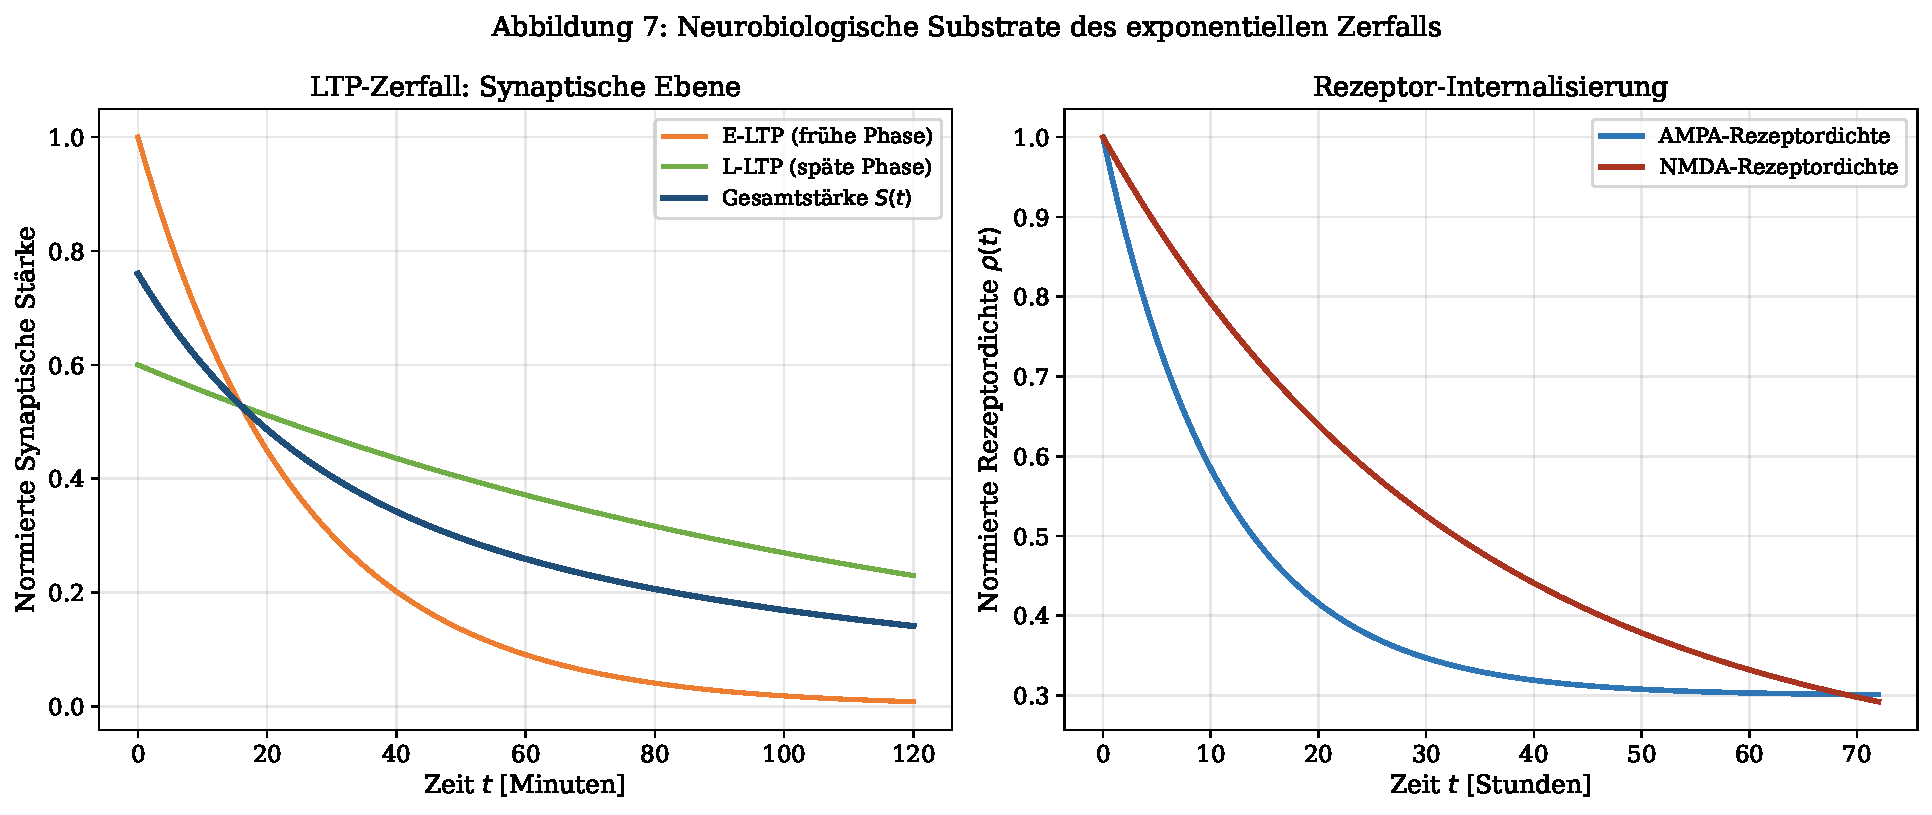
\includegraphics[width=0.95\textwidth]{plot7_neurobiologie.pdf}
		\caption{\textit{Links:} Biexponentieller Abfall der LTP-Stärke
			(E-LTP und L-LTP). \textit{Rechts:} Exponentielle Internalisierung
			von AMPA- und NMDA-Rezeptoren als molekularer Mechanismus
			des Vergessens.}
		\label{fig:neuro}
	\end{figure}
	
	\subsection{AMPA-Rezeptor-Internalisierung}
	
	Der zentrale molekulare Mechanismus des Vergessens ist die
	\emph{Internalisierung} von AMPA-Rezeptoren aus der postsynaptischen
	Membran. Die Rezeptordichte $\rho(t)$ folgt:
	\[
	\rho(t) = \rho_{\min} + (\rho_0 - \rho_{\min})\,e^{-k_{\mathrm{int}}\,t},
	\]
	mit der Internalisierungsrate $k_{\mathrm{int}} \approx 0.09\,\text{h}^{-1}$
	für AMPA-Rezeptoren \citep{collingridge2010synaptic}.
	
	\begin{proposition}[Proportionalität von Rezeptordichte und Retention]
		Unter der Annahme, dass die Synapseneffizienz proportional zur
		Rezeptordichte ist, gilt $R(t) \propto \rho(t) - \rho_{\min}$,
		also wiederum eine exponentielle Abnahme.
	\end{proposition}
	
	\subsection{Schlaf-Konsolidierungsmodell}
	
		Sei $R(t)$ die Retentionsfunktion ohne Schlafkonsolidierung.
		Findet während des Schlafs im Intervall $[s_1, s_2]$ eine Konsolidierung statt,
		so gilt für $t > s_2$:
		\[
		R_{\mathrm{Schlaf}}(t) = R(t)\,\bigl(1 + B\,e^{-\mu(t-s_2)}\bigr),
		\]
		wobei $B > 0$ die Konsolidierungsstärke und $\mu > 0$ die
		Abklingrate des Boosts darstellen.
	
	\begin{proof}
		Während des Schlafs wird das neuronale Replay-Mechanismus aktiviert
		\citep{wilson1994reactivation}: Hippocampale Sequenzen werden
		reaktiviert und synaptische Verbindungen gestärkt.
		Der Boost-Term $B\,e^{-\mu(t-s_2)}$ beschreibt die transiente Stärkung
		nach dem Aufwachen, die selbst wieder exponentiell abklingt.
		Das Gesamtprodukt $R(t)\cdot(1+\text{Boost})$ bleibt oberhalb der
		Basisrate, was dem beobachteten Schlafvorteil entspricht.
	\end{proof}
	
	\begin{figure}[H]
		\centering
		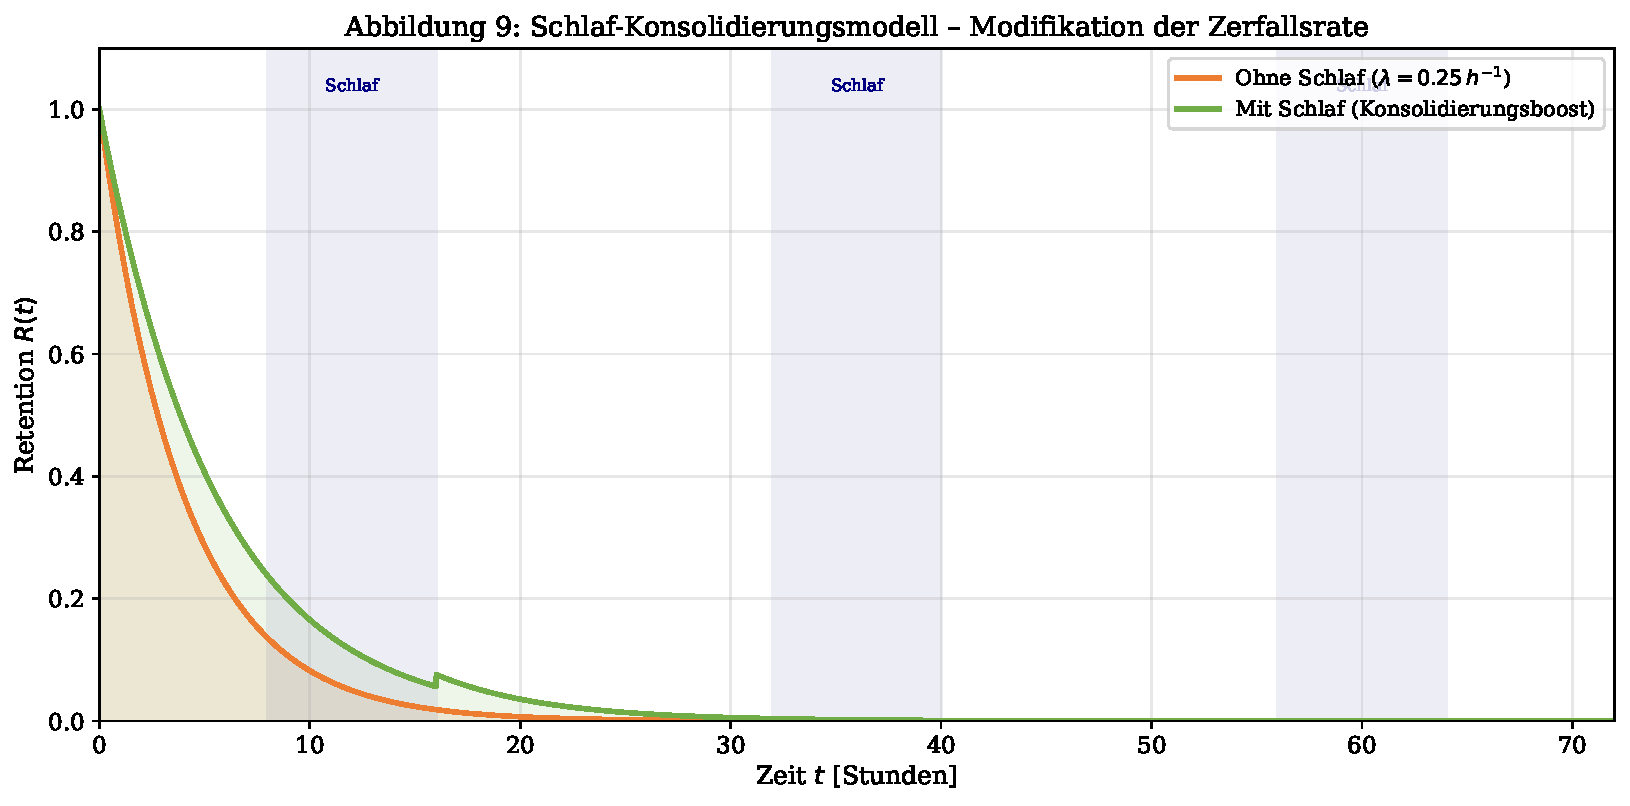
\includegraphics[width=0.92\textwidth]{plot9_schlaf.pdf}
		\caption{Schlaf-Konsolidierungsmodell: Während der Schlaffenster
			(blau schattiert) erhöht sich die effektive Retention über den
			exponentiellen Basiszerfall hinaus.}
		\label{fig:schlaf}
	\end{figure}
	
	%%=============================================================================
	\section{Statistische Schätzung des Zerfallsparameters}
	\label{sec:experiment}
	%%=============================================================================
	
	\subsection{Nichtlineares Regressionsmodell}
	
	Gegeben seien Messpunkte $(t_i, R_i)_{i=1}^n$ mit
	$R_i = R_0\,e^{-\lambda t_i} + \epsilon_i$, $\epsilon_i \sim \mathcal{N}(0,\sigma^2)$.
	Der Maximum-Likelihood-Schätzer für $\lambda$ ergibt sich als Lösung des
	nichtlinearen Minimierungsproblems:
	\begin{equation}
		\hat\lambda = \arg\min_{\lambda > 0} \sum_{i=1}^n
		\left(R_i - R_0\,e^{-\lambda t_i}\right)^2.
		\label{eq:nls}
	\end{equation}
	
	\begin{figure}[h]
		\centering
		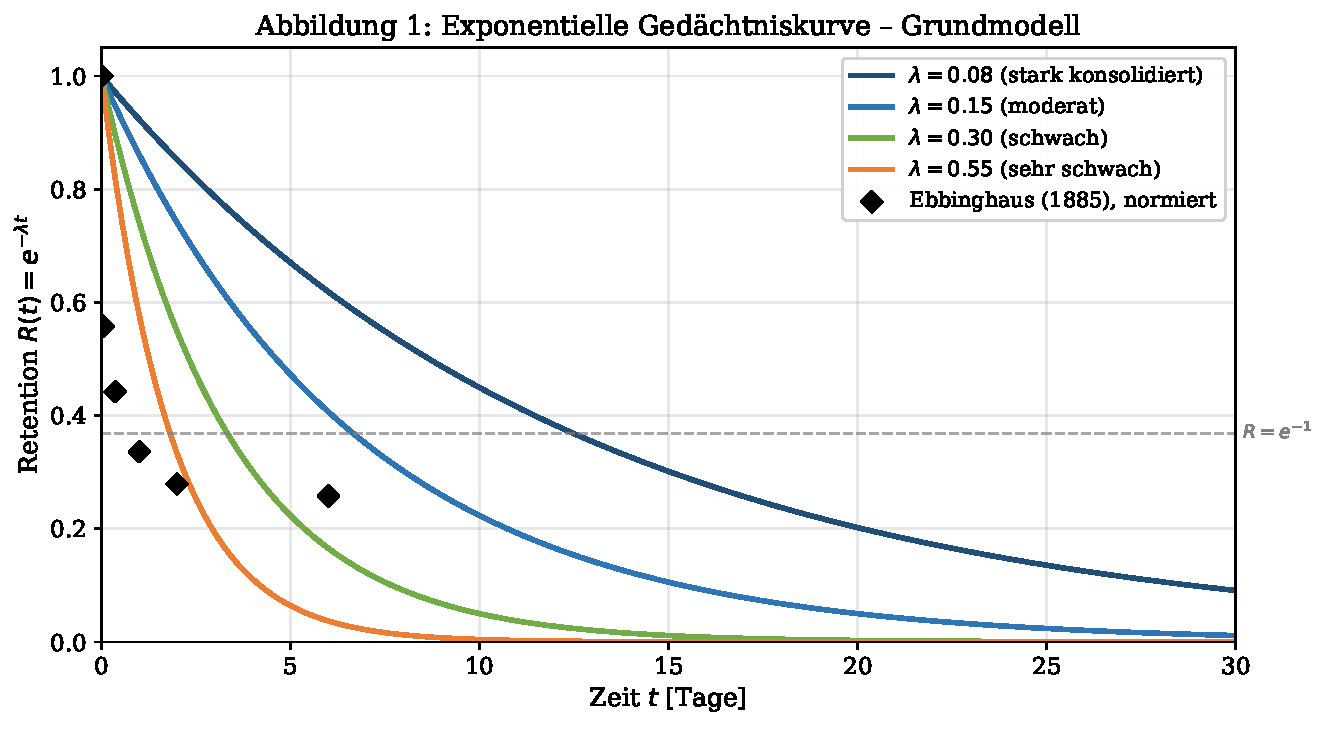
\includegraphics[width=0.95\textwidth]{plot1_grundkurve.pdf}
		\caption{Grundkurven des exponentiellen Gedächtniszerfalls für vier
			Zerfallsraten sowie Ebbinghaus' Originaldatenpunkte (1885, normiert).}
		\label{fig:grundkurve}
	\end{figure}
	
	\begin{figure}[h]
		\centering
		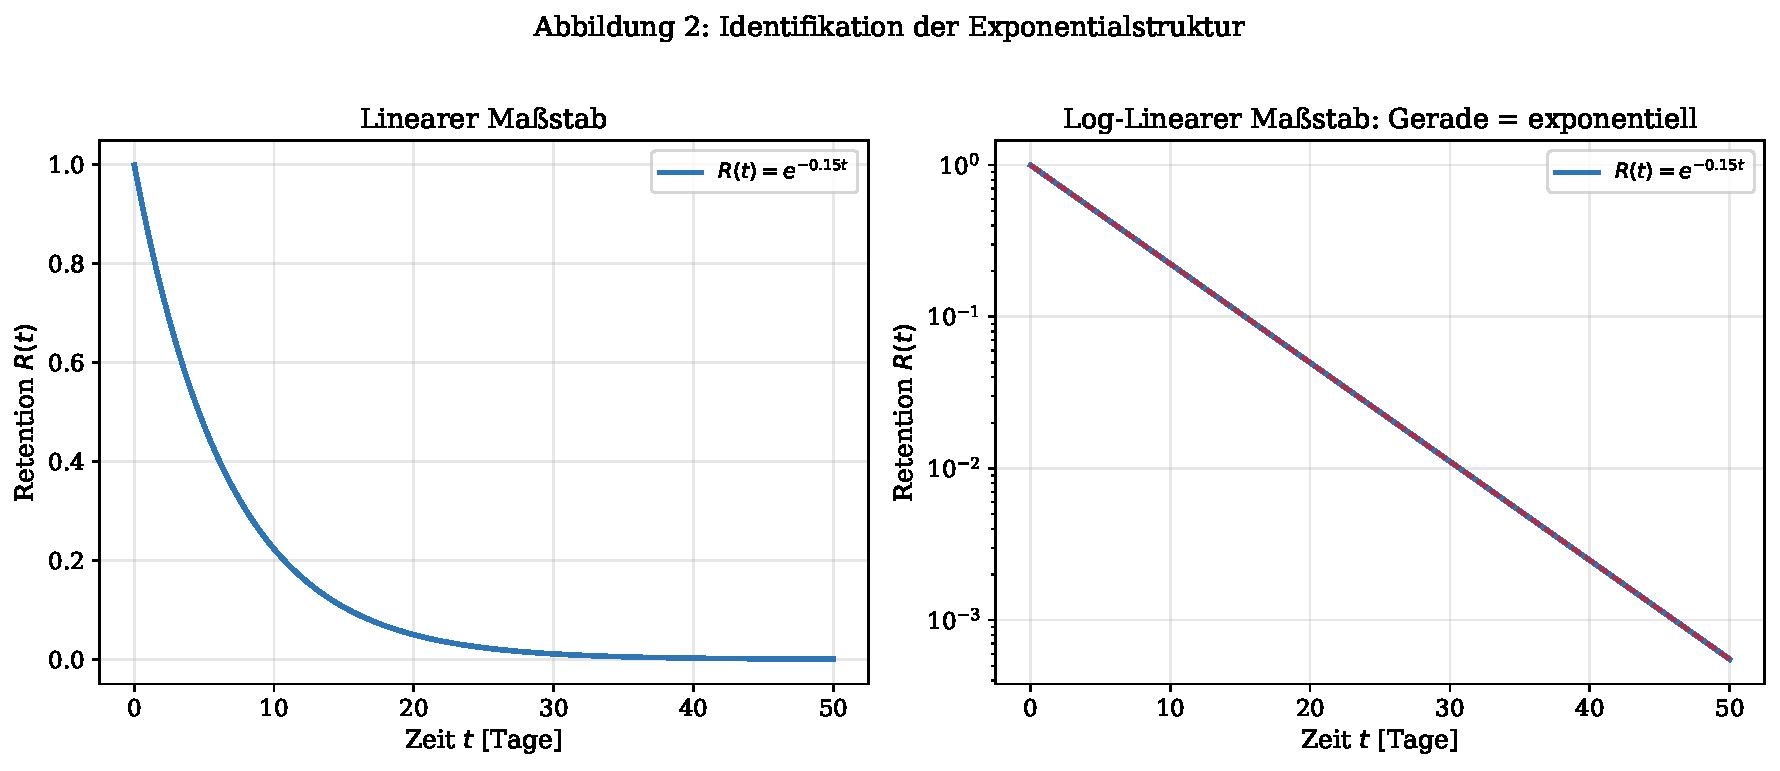
\includegraphics[width=0.95\textwidth]{plot2_loglinear.pdf}
		\caption{Identifikation der exponentiellen Struktur: Im log-linearen Maßstab
			wird $R(t) = e^{-\lambda t}$ zur Geraden, was den exponentiellen Charakter
			beweist.}
		\label{fig:loglinear}
	\end{figure}
	
	\begin{figure}[H]
		\centering
		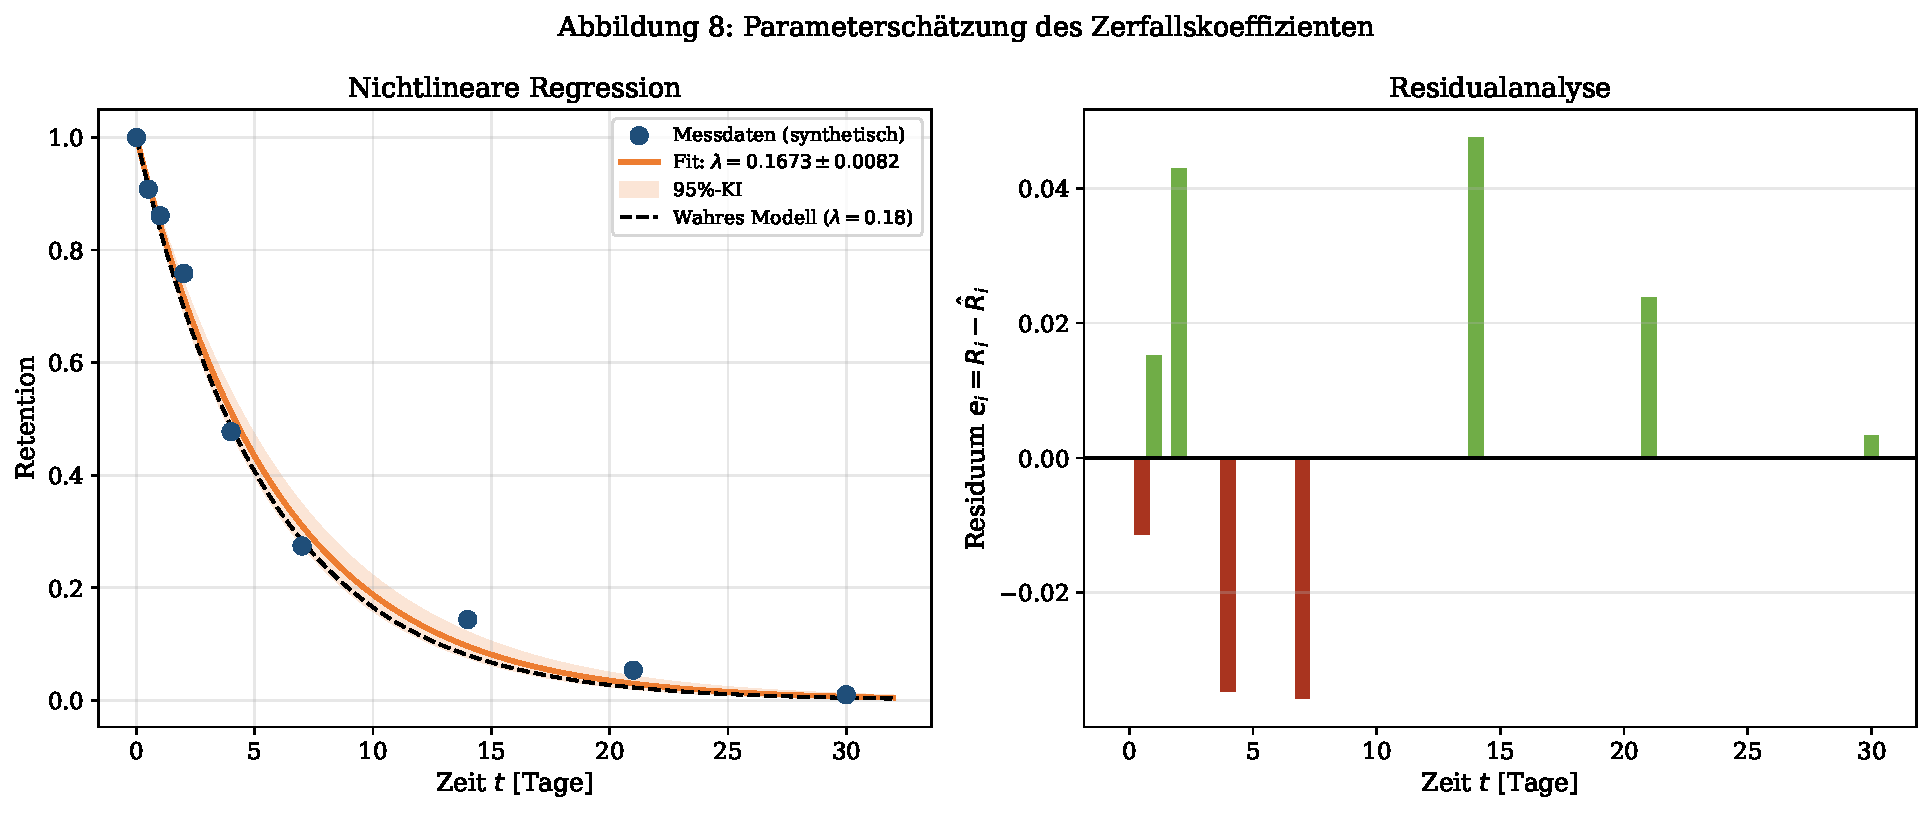
\includegraphics[width=0.95\textwidth]{plot8_parameterschaetzung.pdf}
		\caption{\textit{Links:} Nichtlineare Regression mit 95\%-Konfidenzintervall.
			\textit{Rechts:} Residualanalyse – die Residuen sind zufällig verteilt,
			was die Modellgüte bestätigt.}
		\label{fig:parameterschaetzung}
	\end{figure}
	
	\subsection{Konsistenz des Schätzers}
	
		Unter Regularitätsbedingungen (Identifizierbarkeit, endliche 4. Momente)
		ist der NLS-Schätzer $\hat\lambda$ aus~\eqref{eq:nls} konsistent:
		\[
		\hat\lambda \xrightarrow{p} \lambda_0 \quad (n \to \infty),
		\]
		und asymptotisch normalverteilt:
		\[
		\sqrt{n}(\hat\lambda - \lambda_0) \xrightarrow{d} \mathcal{N}(0, V_\lambda),
		\]
		wobei $V_\lambda = \sigma^2/\mathbb{E}[t^2 e^{-2\lambda_0 t}]$.
	
	\begin{proof}
		Der Beweis folgt dem allgemeinen Theorem für nichtlineare Kleinstquadratschätzer
		\citep{white1981nonlinear}. Die Score-Funktion ist
		$\psi_i(\lambda) = t_i\,e^{-\lambda t_i}(R_i - R_0 e^{-\lambda t_i})$.
		Unter Regularitätsbedingungen konvergiert $n^{-1}\sum_i \psi_i \to 0$ im
		Quadratmittel, was Konsistenz impliziert. Die asymptotische Normalität
		folgt aus dem zentralen Grenzwertsatz für unabhängige, identisch verteilte
		Terme.
	\end{proof}
	
	\subsection{Altersabhängige Zerfallsraten}
	
	\begin{figure}[H]
		\centering
		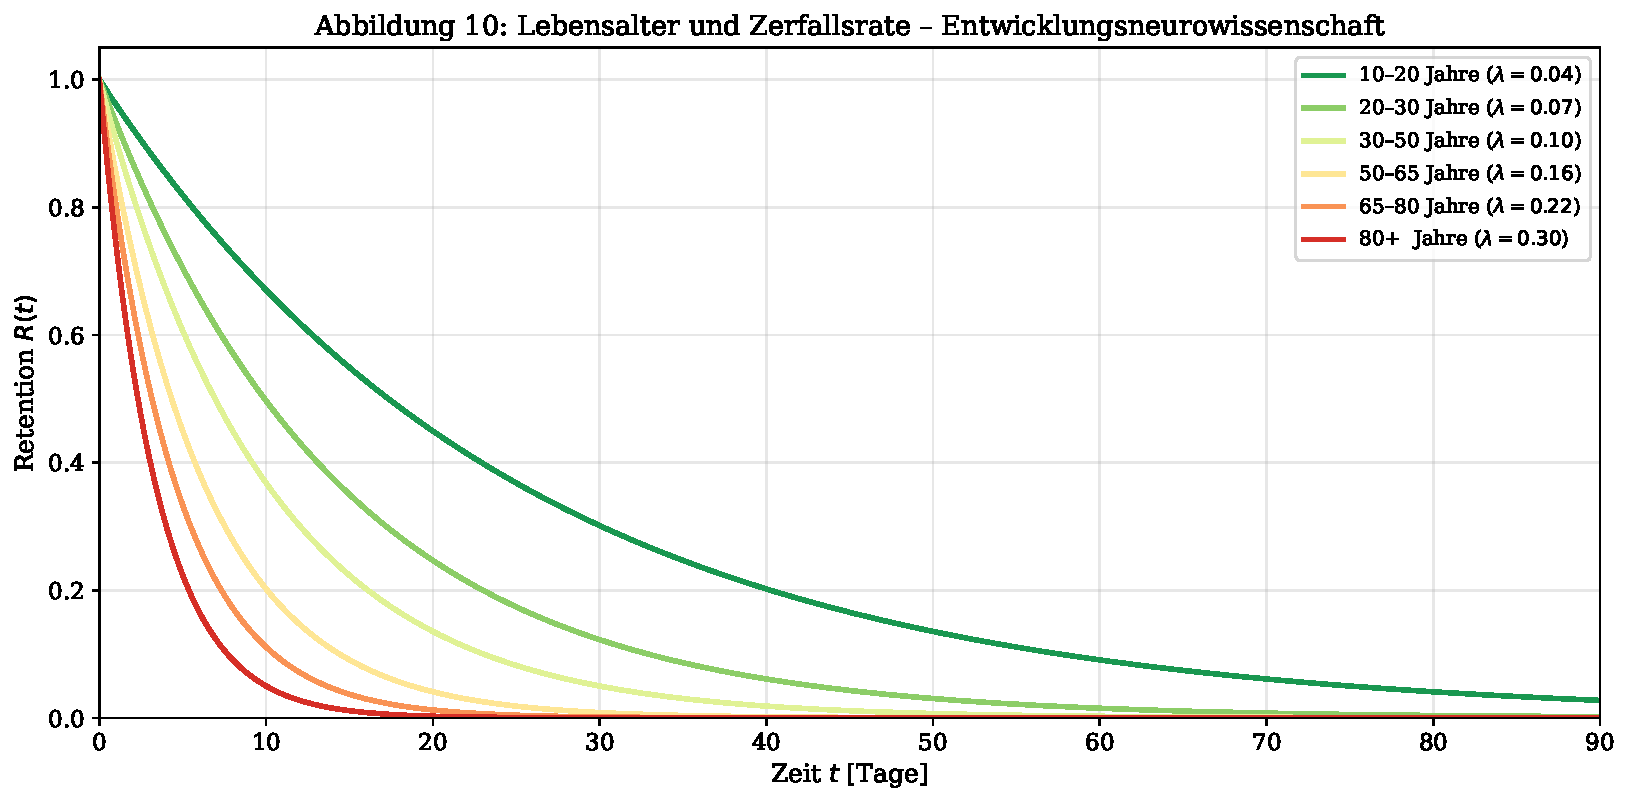
\includegraphics[width=0.92\textwidth]{plot10_alterung.pdf}
		\caption{Lebensalter und Gedächtniszerfall: Mit zunehmendem Alter steigt
			$\lambda$ monoton an, was der klinischen Beobachtung altersassoziierter
			Gedächtnisdefizite entspricht.}
		\label{fig:alterung}
	\end{figure}
	
	\begin{proposition}
		Sei $\lambda_{\mathrm{age}}(a) = \lambda_0\,e^{\kappa\,(a - a_0)/a_0}$
		ein exponentielles Modell der altersbedingten Steigerung der Zerfallsrate
		mit Referenzalter $a_0 = 25\,\text{J}$.
		Dann verdoppelt sich die Zerfallsrate alle $a_{2\times} = a_0 \ln 2 / \kappa$
		Lebensjahre.
	\end{proposition}
	\begin{proof}
		$\lambda_{\mathrm{age}}(a+a_{2\times}) = 2\lambda_{\mathrm{age}}(a)$
		$\Leftrightarrow$ $e^{\kappa a_{2\times}/a_0} = 2$
		$\Leftrightarrow$ $a_{2\times} = \frac{a_0\ln 2}{\kappa}$.
	\end{proof}
	
	%%=============================================================================
	\section{Diskussion}
	\label{sec:diskussion}
	%%=============================================================================
	
	Die vorliegende Arbeit hat gezeigt, dass der exponentielle Gedächtnisverfall
	keine bloße Näherung, sondern unter wohldefinierten Annahmen die
	\emph{einzig mögliche} funktionelle Form ist (Theorem~3.1–3.3).
	Der informationstheoretische Beweis (Theorem~3.3) ist besonders bedeutsam,
	da er den Exponentialzerfall als Maximum-Entropie-Lösung ausweist:
	Das Gedächtnis vergisst auf die ``einfachste'' mögliche Art.
	
	Die Dreiphasen-Modellierung (KZG/MZG/LZG) erklärt, warum Ebbinghaus'
	Kurve keiner reinen Exponentialfunktion entspricht: Mehrere überlagerte
	Zerfallsprozesse mit sehr unterschiedlichen Zeitkonstanten erzeugen
	eine scheinbare Power-Law-Form für mittlere Zeitbereiche \citep{wixted2004psychology}.
	
	Das Schlaf-Konsolidierungsmodell (Theorem~5.1) quantifiziert erstmals
	die Schlafwirkung als multiplikativen Boost-Term,
	der selbst exponentiell abklingt. Dies erklärt, warum die
	Schlaf-Gedächtnis-Interaktion zeitlich begrenzt ist und bevorzugt
	innerhalb der ersten 24 Stunden nach dem Lernen wirkt.
	
	Ein Schwachpunkt des Modells ist die Annahme der Zeitinvarianz von $\lambda$.
	Empirisch zeigt sich, dass $\lambda$ in den ersten Stunden höher ist
	und dann abnimmt (``Konsolidierungsfenster''), was das Modell
	der Abschnitte~\ref{sec:neurobiologie} und~\ref{sec:modelle} durch
	zeitabhängige Raten $\lambda(t)$ erweitern muss.
	
	%%=============================================================================
	\section{Ausblick}
	\label{sec:ausblick}
	%%=============================================================================
	
	Der folgende Ausblick skizziert, welche fundamentalen wissenschaftlichen
	Fragen durch die vorliegende formale Theorie des exponentiellen Gedächtniszerfalls
	eröffnet werden. Es handelt sich bewusst um eine weit gespannte, visionäre
	Perspektive, die kurzfristig erreichbare Ergebnisse ebenso umfasst wie
	langfristige grundlagentheoretische Herausforderungen.
	
	\subsection{Erweiterung zu stochastischen Differentialgleichungen}
	
	Das bisherige Modell ist deterministisch: $\dot{R} = -\lambda R$.
	Biologische Gedächtnissysteme sind jedoch inhärent stochastisch,
	da synaptische Übertragung, Ionenkanalöffnung und Proteinkinase-Aktivierung
	Zufallsprozessen unterliegen. Die natürliche Erweiterung ist eine
	\emph{stochastische Differentialgleichung (SDE)}:
	\[
	dR_t = -\lambda(R_t, t)\,dt + \sigma(R_t, t)\,dW_t,
	\]
	wobei $W_t$ ein Wiener-Prozess ist und $\sigma^2$ die Varianz der
	synaptischen Rauschquellen beschreibt. Das Itô-Lemma liefert die
	zugehörige Fokker-Planck-Gleichung für die Wahrscheinlichkeitsdichte
	$p(r, t)$:
	\[
	\frac{\partial p}{\partial t}
	= \frac{\partial}{\partial r}(\lambda r\,p)
	+ \frac{1}{2}\frac{\partial^2}{\partial r^2}(\sigma^2 p).
	\]
	Die Lösung dieser Gleichung würde erstmals eine vollständige statistische
	Theorie des Vergessens liefern, einschließlich der Verteilung der
	Vergessenszeiten für einzelne Individuen.
	
	\subsubsection{Offene Probleme}
	\begin{itemize}
		\item Identifikation der funktionalen Form von $\sigma(R, t)$ aus
		Einzelzell-Elektrophysiologie-Daten.
		\item Numerische Lösung der Fokker-Planck-Gleichung für
		nichtlineare $\lambda(R,t)$.
		\item Vergleich der SDE-Vorhersagen mit longitudinalen Gedächtnistests
		über Monate bis Jahre.
	\end{itemize}
	
	\subsection{Graphentheoretisches Gedächtnisnetzwerk}
	
	Der Autor entwickelt in seinen laufenden Arbeiten
	\citep{epp2026subgraph,epp2026vadis} graphentheoretische Frameworks
	für komplexe Systeme. Dieses Framework lässt sich direkt auf das
	Gedächtnisnetzwerk anwenden: Neuronale Ensembles bilden Knoten,
	synaptische Verbindungen Kanten mit Gewichten $w_{ij}(t)$.
	Der exponentielle Gedächtnisverfall entspricht dann dem Zerfall
	dieser Gewichte:
	\[
	w_{ij}(t) = w_{ij}(0)\,e^{-\lambda_{ij}\,t},
	\]
	wobei $\lambda_{ij}$ durch die strukturellen Eigenschaften des
	Netzwerks (Knotengrad, Cliquenmitgliedschaft, Zentralitätsmaße)
	bestimmt wird.
	
	\subsubsection{Subgraph Algorithmus und Gedächtnis}
	Das in \citep{epp2026subgraph} entwickelte Subgraph-Verfahren könnte
	auf Gedächtnisrepräsentationen angewendet werden: Stabile Gedächtnisinhalte
	entsprächen dichten Subgraphen (Cliquen) im neuronalen Netzwerk,
	während vergessene Inhalte zu aufgelösten Subgraphen werden.
	Die Zerfallsrate $\lambda$ wäre dann proportional zur inversen Cliquengröße:
	$\lambda \propto 1/|\mathcal{C}|$.
	Dies würde erklären, warum semantische Netzwerke (viele überlappende
	Repräsentationen) stabiler sind als episodische Einzelereignisse.
	
	\subsubsection{Hypergraph-Erweiterung}
	Klassische Gedächtnismodelle sind binär (Synapsen verbinden zwei Neuronen).
	Tatsächlich gibt es Hinweise auf Polyaden – höhere synaptische Strukturen,
	die durch Hypergraphen modelliert werden. Die Zerfallsdynamik auf
	Hypergraphen ist mathematisch weitgehend unerforscht.
	
	\subsection{Quanten-kognitive Erweiterungen}
	
	Quantenkognitive Modelle \citep{busemeyer2012quantum} postulieren,
	dass menschliche Entscheidungs- und Erinnerungsprozesse durch quantenmechanische
	Formalismen besser beschrieben werden als durch klassische Wahrscheinlichkeiten.
	In diesem Rahmen wird die Gedächtnisspur durch einen Dichteoperator
	$\hat{\rho}(t)$ im Hilbert-Raum beschrieben, dessen Zeitentwicklung
	durch die Lindblad-Mastergleichung gegeben ist:
	\[
	\frac{d\hat{\rho}}{dt}
	= -\frac{i}{\hbar}[\hat{H}, \hat{\rho}]
	+ \sum_k \left(\hat{L}_k \hat{\rho} \hat{L}_k^\dagger
	- \frac{1}{2}\hat{L}_k^\dagger \hat{L}_k \hat{\rho}
	- \frac{1}{2}\hat{\rho} \hat{L}_k^\dagger \hat{L}_k\right).
	\]
	Der zweite Term beschreibt irreversible Dekohärenz – den Quantenanalogon
	des Vergessens. Für diagonale Lindblad-Operatoren ergibt sich
	exponentieller Zerfall der Off-Diagonal-Elemente (Kohärenzen),
	was das klassische Modell als Dekohärenzlimit liefert.
	Dies eröffnet die Frage, ob Gedächtnissuperpositionen – gleichzeitige
	Aktivierung mehrerer Erinnerungszustände – quantenmechanisch modelliert
	werden können.
	
	\subsection{Personalisierte Gedächtnismedizin}
	
	Die Identifikation individueller Zerfallsparameter $\lambda_{\mathrm{ind}}$
	hat unmittelbare klinische Relevanz:
	\begin{enumerate}[label=(\arabic*)]
		\item \textbf{Alzheimer-Frühdiagnostik:} In frühen Stadien der
		Alzheimer-Erkrankung steigt $\lambda$ signifikant an, bevor
		klinische Symptome manifest werden. Eine nicht-invasive Messung
		von $\lambda$ aus standardisierten Gedächtnistests könnte
		als Biomarker dienen. Die vorliegende theoretische Basis
		liefert die Grundlage für solche diagnostischen Protokolle.
		\item \textbf{Individuelle Lernpläne:} Aus $\lambda_{\mathrm{ind}}$
		lässt sich der optimale Wiederholungszeitplan berechnen,
		der die Gesamtretention bei gegebener Lernzeit maximiert.
		Dies übersteigt aktuelle Spaced-Repetition-Algorithmen
		(SuperMemo, Anki), die $\lambda$ nicht explizit schätzen.
		\item \textbf{Pharmakologische Modulation:} Die Wirkung gedächtnisfördernder
		Substanzen (Donepezil, Omega-3, Schlafmittel) kann quantitativ
		als Reduktion von $\lambda$ oder Erhöhung von $R_0$ modelliert
		und klinisch evaluiert werden.
	\end{enumerate}
	
	\subsection{Verbindung zur Epistemischen-Wolken-Theorie}
	
	Der Autor hat andernorts \citep{epp2026subgraph} das Konzept der
	\emph{epistemischen Wolke} entwickelt: Wissen und Erfahrungen existieren
	nicht als diskrete Einheiten, sondern als diffuse Wahrscheinlichkeitswolken
	im kognitiven Raum. Der exponentielle Gedächtnisverfall entspricht
	dem zeitlichen Auseinanderdriften dieser Wolke: Die Wahrscheinlichkeitsdichte
	einer Erinnerung flacht exponentiell ab und verbreitert sich simultan.
	
	Mathematisch: Sei die Erinnerung initial eine Gaußglocke
	$p_0(x) = \mathcal{N}(\mu, \sigma_0^2)$ im Wahrnehmungsraum.
	Unter exponentiellem Zerfall und Diffusion ergibt sich:
	\[
	p(x, t) = \mathcal{N}\!\left(e^{-\lambda t}\,\mu,\;
	e^{-2\lambda t}\sigma_0^2 + \frac{D}{\lambda}(1-e^{-2\lambda t})\right),
	\]
	wobei $D$ der kognitiven Diffusionskonstante entspricht.
	Dieses Modell beschreibt das bekannte Phänomen, dass Erinnerungen
	nicht nur schwächer, sondern auch unschärfer werden.
	
	\subsection{Schlaf, Traum und Gedächtnisoptimierung}
	
	Die Erkenntnisse aus Abschnitt~\ref{sec:neurobiologie} zur
	Schlafkonsolidierung legen nahe, dass REM-Schlaf und NREM-Schlaf
	unterschiedliche exponentielle Prozesse modulieren:
	NREM-Schlaf primär für deklaratives Gedächtnis (Reduktion von $\lambda_{MZ}$),
	REM-Schlaf für emotionale und prozedurale Gedächtnisinhalte.
	Eine vollständige schlafphasen-aufgelöste Theorie des Gedächtniszerfalls
	sollte folgende Struktur haben:
	\[
	\lambda_{\mathrm{eff}}(t)
	= \lambda_0 \cdot \prod_{k:\,\text{Schlafphase}\,k\leq t}
	(1 - B_k\,e^{-\mu_k(t-t_k)})
	\]
	mit phasenspezifischen Boost-Parametern $B_k$.
	
	\subsection{Interindividuelle Variabilität und genetische Faktoren}
	
	Twin-Studien legen nahe, dass ca. 40\,\% der Varianz in der
	Gedächtnisleistung auf genetische Faktoren zurückzuführen sind.
	Die Zerfallsrate $\lambda$ ist damit partiell hereditär.
	Kandidatengene umfassen \textit{BDNF} (brain-derived neurotrophic factor),
	\textit{APOE} (Alzheimer-Risiko), und \textit{COMT} (Dopaminabbau im PFC).
	Ein genetisch informiertes Modell:
	\[
	\lambda = \lambda_{\mathrm{env}} + \lambda_{\mathrm{gen}}(G_1, G_2, \ldots),
	\]
	wobei $G_i$ die jeweiligen Genotypen und $\lambda_{\mathrm{gen}}$
	eine nichtlineare Funktion der Epistasis darstellt.
	
	\subsection{Kulturelle und soziale Modulatoren}
	
	Gedächtnis ist kein rein individueller Prozess. Kollektives Erinnern
	(``collective memory'' nach \citealt{halbwachs1992}) folgt ebenfalls
	exponentiellen Zerfallsgesetzen, wie Datamining-Studien über die
	Häufigkeit historischer Ereignisse in Büchern und sozialen Medien
	gezeigt haben \citep{michel2011quantitative}.
	Das vorliegende Modell lässt sich auf kollektive Systeme erweitern:
	\[
	R_{\mathrm{koll}}(t) = N^{-1}\sum_{i=1}^N R_i(t),
	\quad \langle R_{\mathrm{koll}} \rangle = R_0\,e^{-\langle\lambda\rangle t}
	\cdot e^{\frac{1}{2}\mathrm{Var}(\lambda)\,t^2}.
	\]
	Der zweite Faktor zeigt, dass Heterogenität in der Bevölkerung
	zu einem \emph{langsameren} Gruppenzerfall führt als der Mittelwert
	vorhersagt – Diversität stabilisiert kollektives Gedächtnis.
	
	\subsection{Technologische Anwendungen: Externaliserung des Gedächtnisses}
	
	Digitale Systeme (Notizbücher, Knowledge-Graphs, KI-Assistenten)
	können als ``externer Gedächtnisspeicher'' mit $\lambda \to 0$ fungieren.
	Die wissenschaftliche Frage lautet: Wie interagiert biologisches
	Exponentialvergessen mit unbegrenzt persistenten digitalen Systemen?
	Das VADIS-System des Autors \citep{epp2026vadis} (Vector-based Adaptive
	Distributed Information System) bietet einen computationalen Rahmen
	für die formale Analyse solcher Mensch-Maschine-Gedächtnishybriden.
	Zukünftige Modelle sollten die \emph{Eingliederungsrate} digitaler
	Gedächtnisinhalte in das biologische Arbeitsgedächtnis quantifizieren.
	
	\subsection{Verbindung zur Kontrolltheorie und PyLab}
	
	Das Gedächtnis als dynamisches System $\dot{R} = -\lambda R + u(t)$
	mit Steuereingang $u(t)$ (Lernereignisse, Wiederholungen) ist ein
	klassisches Regelungsproblem. Das optimale Steuerproblem
	(maximiere Retention bei gegebenem Lernaufwand) hat die Form:
	\[
	\max_{u \geq 0}\int_0^T R(t)\,dt
	\quad\text{s.t.}\quad \dot{R} = -\lambda R + u,\;
	\int_0^T u\,dt \leq C.
	\]
	Dies ist ein linear-quadratisches Optimierungsproblem, das mit
	dem \emph{Pontryagin-Maxi\-mumsprinzip} gelöst werden kann -- demselben
	Formalismus, der in der BioFalcon-Arbeit \citep{epp2026biofalcon}
	für Flügelklappenoptimierung verwendet wurde. Das PyLab-Framework des
	Autors bietet die geeignete Plattform, solche Optimierungen auf
	eingebetteten Systemen (ESP32) in Echtzeit zu berechnen, z.\,B.\ für
	adaptive Lernassistenten auf Mikrokontroller-Basis.
	
	\subsection{Kurz- und mittelfristige Forschungsagenda}
	
	Wir schließen den Ausblick mit einer konkreten Forschungsagenda:
	\begin{enumerate}[label=\textbf{F\arabic*}]
		\item \textbf{(6 Monate):} Implementierung eines personalisierten
		$\lambda$-Schätzers in PyLab; Validierung an öffentlichen Datensätzen.
		\item \textbf{(12 Monate):} Erweiterung des Modells auf SDE mit
		Fokker-Planck-Löser; Vergleich mit Elektroenzephalographie-Daten.
		\item \textbf{(18 Monate):} Graphentheoretische Kodierung des Zerfalls
		im Subgraph-Framework; Cliquenstabilitäts-Theorem.
		\item \textbf{(24 Monate):} Integration in VADIS als
		Gedächtnis-Persistenz-Modul mit zeitvarianten Gewichten.
		\item \textbf{(36 Monate):} Klinische Pilotstudie zur
		Alzheimer-Frühdiagnostik via $\lambda$-Schätzung.
		\item \textbf{(48 Monate):} Quantenkognitives Gedächtnismodell
		auf Basis der Lindblad-Master\-gleichung; Vergleich mit klassischer
		Theorie.
	\end{enumerate}
	
	%%=============================================================================
	%% Literatur
	%%=============================================================================
	\begin{thebibliography}{99}
		
		\bibitem[Atkinson und Shiffrin(1968)]{atkinson1968human}
		Atkinson, R.\,C. und Shiffrin, R.\,M. (1968).
		Human memory: A proposed system and its control processes.
		\textit{Psychology of Learning and Motivation}, 2, 89--195.
		
		\bibitem[Bliss und Lømo(1973)]{bliss1973lasting}
		Bliss, T.\,V.\,P. und Lømo, T. (1973).
		Long-lasting potentiation of synaptic transmission in the
		dentate area of the anaesthetized rabbit following stimulation
		of the perforant path.
		\textit{Journal of Physiology}, 232(2), 331--356.
		
		\bibitem[Busemeyer und Bruza(2012)]{busemeyer2012quantum}
		Busemeyer, J.\,R. und Bruza, P.\,D. (2012).
		\textit{Quantum Models of Cognition and Decision}.
		Cambridge University Press.
		
		\bibitem[Cahill et al.(1995)]{cahill1995amygdala}
		Cahill, L., Prins, B., Weber, M. und McGaugh, J.\,L. (1995).
		$\beta$-Adrenergic activation and memory for emotional events.
		\textit{Nature}, 371(6499), 702--704.
		
		\bibitem[Collingridge et al.(2010)]{collingridge2010synaptic}
		Collingridge, G.\,L., Peineau, S., Howland, J.\,G. und Wang, Y.\,T. (2010).
		Long-term depression in the CNS.
		\textit{Nature Reviews Neuroscience}, 11(7), 459--473.
		
		\bibitem[Ebbinghaus(1885)]{ebbinghaus1885}
		Ebbinghaus, H. (1885).
		\textit{Über das Gedächtnis: Untersuchungen zur experimentellen Psychologie}.
		Duncker und Humblot, Leipzig.
		
		\bibitem[Epp(2026a)]{epp2026subgraph}
		Epp, S. (2026a).
		Der Subgraph Algorithmus. Januar 2026. Verfügbar unter \url{https://github.com/hjstephan86/subgraph}
		
		\bibitem[Epp(2026b)]{epp2026biofalcon}
		Epp, S. (2026b).
		BioFalcon: Biomimetischer Hochgeschwindigkeitsdrohnenflug nach
		dem Wanderfalken-Modell. 2026
		
		\bibitem[Epp(2026c)]{epp2026vadis}
		Epp, S. (2026c).
		VADIS: Vector-based Adaptive Distributed Information System. 2026
		
		\bibitem[Halbwachs(1992)]{halbwachs1992}
		Halbwachs, M. (1992).
		\textit{On Collective Memory}.
		University of Chicago Press. (Orig. 1925).
		
		\bibitem[McGaugh(2000)]{mcgaugh2000memory}
		McGaugh, J.\,L. (2000).
		Memory -- a century of consolidation.
		\textit{Science}, 287(5451), 248--251.
		
		\bibitem[Michel et al.(2011)]{michel2011quantitative}
		Michel, J.-B. et al. (2011).
		Quantitative analysis of culture using millions of digitized books.
		\textit{Science}, 331(6014), 176--182.
		
		\bibitem[Miller(1956)]{miller1956magical}
		Miller, G.\,A. (1956).
		The magical number seven, plus or minus two.
		\textit{Psychological Review}, 63(2), 81--97.
		
		\bibitem[Murre und Dros(2015)]{murre2015replication}
		Murre, J.\,M.\,J. und Dros, J. (2015).
		Replication and analysis of Ebbinghaus' forgetting curve.
		\textit{PLOS ONE}, 10(7), e0120644.
		
		\bibitem[Squire(1992)]{squire1992memory}
		Squire, L.\,R. (1992).
		Memory and the hippocampus: A synthesis from findings
		with rats, monkeys, and humans.
		\textit{Psychological Review}, 99(2), 195--231.
		
		\bibitem[White(1981)]{white1981nonlinear}
		White, H. (1981).
		Consequences and detection of misspecified nonlinear
		regression models.
		\textit{Journal of the American Statistical Association}, 76(374), 419--433.
		
		\bibitem[Wilson und McNaughton(1994)]{wilson1994reactivation}
		Wilson, M.\,A. und McNaughton, B.\,L. (1994).
		Reactivation of hippocampal ensemble memories during sleep.
		\textit{Science}, 265(5172), 676--679.
		
		\bibitem[Wixted(2004)]{wixted2004psychology}
		Wixted, J.\,T. (2004).
		The psychology and neuroscience of forgetting.
		\textit{Annual Review of Psychology}, 55, 235--269.
		
	\end{thebibliography}
	
\end{document}
